\begin{figure}[t]
%
\centering
\begin{tabular}{c@{\hfill}c}
%
\begin{minipage}[t]{.5\textwidth}
\[
\begin{array}{ll}
\num{1}~ & ~~ \esc{write}\ (p,\, v)\ \{\\ 
\num{2}~ & ~~~~~ \lat\,\actwrite{p}{v}; \aux{register}(p,v)\rat;\\
\num{3}~ & ~~~~~ \lat\, b \tbnd \act{read}(S);\ \aux{check}(p,b) \rat;\\
\num{4}~ & ~~~~~ \kw{if}\ b\\
\num{5}~ & ~~~~~ \kw{then}\ \lat\,%
                           \actwrite{\aleksfwdp{p}}{v};\ \aux{forward}(p)\rat; \\
\num{5'}~           & ~~~~ \lat\,\aux{finalize}(p)\rat\}
\end{array}
\]
\end{minipage}
%
&
%
\begin{minipage}[t]{.5\textwidth}
\[
\begin{array}{rl}
\num{6}~  & \esc{scan} () : ( A \times A )~ \{ \\ 
\num{7}~  & ~~~ \lat\,\actwrite{\s}{\esc{true}};\ \aux{set}(\esc{true}) \rat;\\  
\num{8}~  & ~~~ \lat\,\actwrite{\fx}{\bot};\ \aux{clear}(\x)\rat;\\
\num{9}~  & ~~~ \lat\,\actwrite{\fy}{\bot};\ \aux{clear}(\y)\rat;\\
\num{10}~ & ~~~ \var{vx} \tbnd \lat \act{read}(\x) \rat ; \\
\num{11}~ & ~~~ \var{vy} \tbnd \lat \act{read}(\y) \rat;  \\
\num{12}~ & ~~~ \lat\,\actwrite{\s}{\esc{false}};\ \aux{set}(\esc{false})\rat;\\
\num{13}~ & ~~~ \var{ox} \tbnd \lat \act{read}(\fx) \rat;\\
\num{14}~ & ~~~ \var{oy} \tbnd \lat \act{read}(\fy) \rat;\\
\num{15}~ & ~~~ \var{rx} \tbnd \kw{if}\ (\var{ox} \neq\bot)\
                \kw{then}\ \var{ox}\ \kw{else}\ \var{vx};\\
\num{16}~ & ~~~ \var{ry} \tbnd \kw{if}\ (\var{oy} \neq\bot)\
                \kw{then}\ \var{oy}\ \kw{else}\ \var{vy};\\
\num{17~} & ~~~ \lat\,\aux{relink}(\var{rx}, \var{ry});\
                \kw{return}\ (\var{rx}, \var{ry})\,\rat\}
\end{array}
\]
\end{minipage}
%
\end{tabular}
%
\caption{Snapshot procedures annotated with auxiliary code.}
\label{fig:fcsl-snapshot}
\end{figure}




\section{Auxiliary code implementation}
\label{sc:implementation}

%\paragraph*{Implementation}%

Figure~\ref{fig:fcsl-snapshot} annotates Jayanti's procedures with
auxiliary code (typed in \emph{italic}), with $\langle\mbox{angle
braces}\rangle$ denoting that the enclosed real and auxiliary code
execute \emph{simultaneously} (\ie, atomically). The auxiliary code
builds the histories, evolves the sequence $\ordlist$, and updates the
color of various write events, while respecting the invariants from
Section~\ref{sc:formal}. Thus, it is the \emph{constructive} component
of our proofs. Each atomic command in Figure~\ref{fig:fcsl-snapshot}
represents one \emph{transition} of the STS $C$ from
Figure~\ref{fig:specs}.

%
%As customary, auxiliary code is \emph{erasable} at run time; it does
%not mutate the real state.
%
%% We name auxiliary code as one would name procedure calls, and proceed
%% to describe these procedures.
%

The auxiliary code is divided into several procedures, all of which
are sequences of reads followed by updates to auxiliary variables. We
present them as Hoare triples in Figure~\ref{fig:auxcode}, with the
unmentioned state considered unchanged. The bracketed variables
preceding the triples (\eg, $[t, v]$) are logical variables used to
show how the pre-state value of some auxiliary changes in the
post-state. To symbolize that these triples \emph{define} an atomic
command, rather than merely stating the command's properties, we
enclose the pre- and postcondition in angle brackets $\langle
- \rangle$.

%Following are the characteristic cases.

% %%\usetikzlibrary{arrows,shapes,automata, positioning}
\usetikzlibrary{arrows,shapes,automata,positioning}

%% \begin{figure}[ht]
%% \begin{subfigure}[t]{.4\textwidth}
%% \centering
%% \small
%% \begin{tikzpicture}[->,>=stealth',shorten >=1pt,auto,node distance=3cm,
%%                     thick,initial text={},initial above]
%%   \tikzstyle{every state}=[fill=white,draw,ellipse,text=black]
%%   \node[initial,state] (A)                    {$\mathsf{Init}$};
%%   \node[state]         (B) [below right of=A] {$\mathsf{Written\ t}$};
%%   \node[state]         (D) [below left of=A] {$\mathsf{Clean\ t}$};
%%   \node[state]         (C) [below left of=B] {$\mathsf{Dirty\ t}$};
 
%%   \path (A) edge [bend left]  node {$\act{register}(p,v)$} (B)
%%         (B) edge [bend left]  node {$\act{check}(p,true)$} (C)
%%             edge              node {$\act{check}(p,false)$} (D)
%%         (C) edge [bend left]  node {$\act{forward}(p)$}(D)
%%         (D) edge [bend left]  node {$\act{exit}()$} (A);
%% \end{tikzpicture}
%% \caption{\label{fig:sts:writer} Write STS on $\wstate{p}$}
%% \end{subfigure}%
%% \begin{subfigure}[t]{.6\textwidth}
%% \centering
%% \small
%% \begin{tikzpicture}[->,>=stealth',shorten >=1pt,auto,node distance=2.2cm,
%%                     thick,initial text={},]
%%   \tikzstyle{every state}=[fill=white,draw,ellipse,text=black]
%%   \node[initial,state] (A)                     {$(\FF,\FF,\FF)$};
%%   \node[state]         (B)  [above right of=A] {$(\TT,\FF,\FF)$};
%%   \node[state]         (C1) [above right of=B] {$(\TT,\TT,\FF)$};
%%   \node[state]         (C2) [below right of=B] {$(\TT,\FF,\TT)$};
%%   \node[state]         (D)  [right=2.5 cm of B]  {$(\TT,\TT,\TT)$};
%%   \node[state]         (E)  [below right=0.5cm and 0.cm of C2]
%%                               {$(\FF,\TT,\TT)$};
%%   \path (A)  edge [bend left]   node {$\act{set}(\TT)$} (B)
%%         (B)  edge [bend left]   node {$\act{clear}(\mathtt{x})$} (C1)
%%              edge [bend right]  node {$\act{clear}(\mathtt{y})$} (C2)
%%         (C1) edge [bend left]   node {$\act{clear}(\mathtt{y})$} (D)
%%         (C2) edge [bend right]  node {$\act{clear}(\mathtt{x})$} (D)
%%         (D)  edge [bend left]   node {$\act{set}(\FF)$} (E)
%%         (E)  edge [bend left]   node {$\act{relink}(rx,ry)$} (A);
%% \end{tikzpicture}
%% \caption{\label{fig:sts:scanner} Scan STS on $\wstate{S}$}
%% \end{subfigure}
%%  \caption{\label{fig:sts} The State Transition System described by auxiliary code}
%% \end{figure}

% I don't need the scanner protocol at all
%\begin{figure}

\begin{figure}
\small
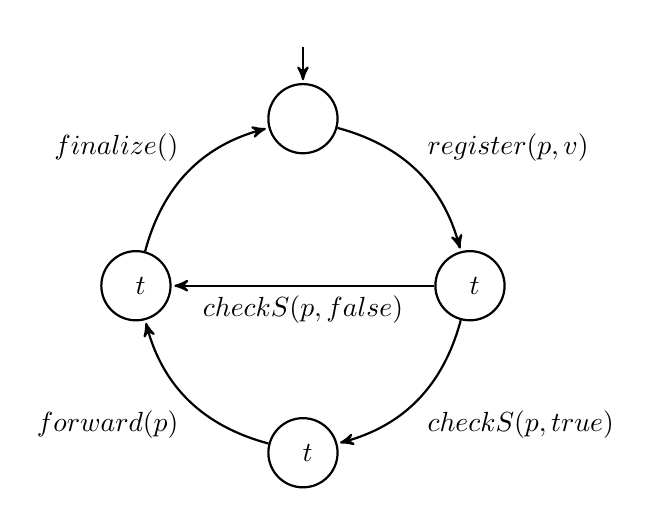
\begin{tikzpicture}[->,>=stealth',shorten >=1pt,auto,node distance=3cm,
                    thick,initial text={},initial above]
  \tikzstyle{every state}=[fill=white,draw,ellipse,text=black]
  \node[initial,state] (A)                    {$\wInit$};
  \node[state]         (B) [below right of=A] {$\wWrite\ t$};
  \node[state]         (D) [below left of=A] {$\wClean\ t$};
  \node[state]         (C) [below left of=B] {$\wDirty\ t$};
 
  \path (A) edge [bend left]  node {$\act{register}(p,v)$} (B)
        (B) edge [bend left]  node {$\act{checkS}(p,true)$} (C)
            edge              node {$\act{checkS}(p,false)$} (D)
        (C) edge [bend left]  node {$\act{forward}(p)$}(D)
        (D) edge [bend left]  node {$\act{finalize}()$} (A);
\end{tikzpicture}
\caption{\label{fig:sts-writer} \jywrite's auxiliary code implements a STS on writer states $\wpp$.}
\end{figure}

\begin{figure}
\small
\begin{tikzpicture}[->,>=stealth',shorten >=1pt,auto,node distance=2cm,
                    thick,initial text={},]
  \tikzstyle{every state}=[fill=white,draw,ellipse,text=black]

  \node[] (I) [] {};
  \node[] (X) [above=1.5 cm of I] {}; 
  \node[state]         (B)  [left=0.5 cm of X]  {$(\sOn,\FF,\FF)$};
  \node[state]         (C)  [right=0.5 cm of X] {$(\sOn,\TT,\FF)$};
  \node[initial,state] (A)  [left= 1.5 cm of I] {$(\sOff\ \_,\FF,\FF)$};
  \node[state]         (D)  [right= 1.5 cm of I] {$(\sOn,\TT,\TT)$};
  \node[state]         (E)  [below=1 cm of I] {$(\sOff\ t,\TT,\TT)$};

\path (A)  edge [bend left]   node {$\act{setS}(\esc{true})$} (B)
        (B)  edge [bend left=10]   node {$\act{clear}(\x)$} (C)
        (C)  edge [bend left]  node {$\act{clear}(\y)$} (D)
        (D)  edge [bend left]   node {$\act{set}(\esc{false})$} (E)
        (E)  edge [bend left]   node {$\act{relink}(rx,ry)$} (A);
\end{tikzpicture}

\caption{\label{fig:sts-scan}%
\jyscan's auxiliary code implements a STS on scanner states $(\spp, \sx, \sy)$.}

\end{figure}



{
%\setlength{\belowcaptionskip}{-5pt}
\begin{figure}[t]
%
\centering
%\begin{subfigure}[t]{1\textwidth}
\small
\[
\begin{array}{l@{\, :\ } l}
%% register
 \aux{register}(p,v) & 
  \begin{array}[t]{l}
   \langle \wpp = \wInit\rangle\\ 
   \langle\ordlistP = \mathsf{snoc}\ {\ordlist}\ t,\
     \histJP = \histJ \hunion t \hpts (p,v),\ \wppP = \wWrite\ t\, v,\\
   \phantom{\langle} \C' = \textrm{if}\ (\sss = \sOn) \& \spp\
                    \textrm{then}\ \C[t \mapsto \mathsf{yellow}]\
                    \textrm{else}\ \C[t \mapsto \mathsf{red}]\rangle \\
   \ \mbox{\small{where $t = \mathsf{fresh}\ \hist = \mathsf{last}\ {\hist}+1$}}
%c \hunion
%(t \mapsto \textrm{if}\ \s \& \spp\ \textrm{then}\ \mathsf{green}\
%\textrm{else}\ \mathsf{yellow})\}\quad\mbox{where $t = \mathsf{fresh}\ \hist$}
  \end{array} \\[2.5pt]
%% checkS
% Im placing it within an  array env so it aligns nicely with the rest
  \aux{check}\,(p,b) & [t, v]\ldot
  \!\begin{array}[t]{l}
  \langle\wpp = \wWrite\ t\, v\rangle\ 
  \langle\wppP = \textrm{if}\ b\
  \textrm{then}\ \wDirty\ t\, \,v\ \textrm{else}\ \wClean\ t\, v\rangle
 \end{array}\\[2.5pt]
%% transfer   
  \aux{forward}\,(p) & [t, v]\ldot
  \!\begin{array}[t]{l}
   \langle\wpp = \wDirty\ t\,v \rangle\\ 
   \langle\wppP = \wClean\ t\,v,\, %
   \C' = \textrm{if}\ (\sss=\sOn) \& \spp\ \textrm{then}\ \C[t \mapsto \mathsf{green}]\ \textrm{else}\ \C\rangle
  \end{array}\\[2.5 pt]
%% exit  
  \aux{finalize}(p) & [t, v]\ldot
  \!\begin{array}[t]{l}
  \langle\wpp = \wClean\ t\, v, %
  t \hpts (p, v) \in \histJ \rangle\\
  \langle\wppP = \wInit,\, \histSP = \histS \hunion t \hpts (p,v),\, %
  \histJP\! = \histJ\setminus\{t\},\,
  \E'\! = \E \hunion\! t \hpts \mathsf{last}\, \hist \rangle
 \end{array}
\end{array}
\]
%\caption{\label{fig:writeauxcode}}
\hrulefill
%\end{subfigure}
%
%\begin{subfigure}[b]{1\textwidth}
\small
\[
\begin{array}{l@{\, :\ }l}
%% setbit
  \aux{set}(b) &
  \begin{array}[t]{l}
        \langle \sss = \textrm{if}\ b\ \textrm{then}\ \sOff\,(\_) \ 
        \textrm{else}\ \sOn,\ \sx = \neg\, b, \sy = \neg\, b \rangle\\
        \langle \sss' = \textrm{if}\ b\ \textrm{then}\ \sOn\ %
        \textrm{else}\ \sOff\,(\mathsf{last}\ \hist),\
         \sx' = \neg\, b, \sy' = \neg\, b \rangle
\end{array}\\[2.5pt] 
%% clear
   \aux{clear}(p) &
  \begin{array}[t]{l}
   \langle\sss = \sOn,\ \spp = \FF \rangle\\
   \langle\sss' = \sOn,\ \spp' = \TT,\
     \CP = \C[\histp \hpts \mathsf{green}] \rangle
  \end{array}\\[2.5pt]
%% re-link
   \aux{relink}(r_x, r_y) & [t_x, t_y]\ldot
    \begin{array}[t]{l}
    \langle\sss = \sOff(\_), %
      t_x \hpts (x, r_x), t_y \hpts (y, r_y) \in \hist, \sx = \sy = \TT, \\
%      \ p \in \{x,y\}:\ \spp =\TT, (t_p = \aux{last\_green}\ \histp \vee
%                \C(t_p) = \mathsf{yellow})\}\\
     \hphantom{\langle} \forall p \in \{x,y\}\ldot \lgVy\ p\, t_p \rangle\\
        \langle\sss' = \sss, \sx'= \sy'=\FF,%
        \CP = \C[t_x, t_y \hpts \mathsf{green}],\\
      \ \ordlist' = \textrm{if}\ (d = \mathsf{Yes}\ x\ s)\
                \textrm{then}\ \aux{push}\ s\ t_y\ \ordlist\\
                 \phantom{\ \ordlist =\ } \textrm{else\ if}\
                 (d = \mathsf{Yes}\ y\ s)\ \textrm{then}\
                 \aux{push}\ s\ t_x\ \ordlist\ \textrm{else}\ \ordlist\rangle\\
  \quad \mbox{where $d = \aux{inspect}\ t_x\, t_y\, \ordlist\, \C$}
  \end{array}
\end{array}
\]
%\caption{\label{fig:scanauxcode}}
%\end{subfigure}
\caption{\label{fig:auxcode} Auxiliary procedures for
%  (\subref{fig:writeauxcode}) 
\jywrite~and 
%(\subref{fig:scanauxcode})
  \jyscan. Bracketed variables (\eg, $[t, v]$) are logical variables
  that scope over precondition and postcondition.}
\end{figure}
}

%\gad{I'm not sure we want to keep the $(t_p =
%  \aux{last\_green}\ \histp \vee \C(t_p) = \mathsf{yellow})$ part, as
%  it is not the pre-variable relating to some auxiliary state
%  projection. This will appear later in the pre and post condition of
%  the atomic commands so it seems repetitive here. Note that the
%  ACTUAL implementation does take a proof that the values are pointed
%  by the last green or yellow timestamp, but there is no need to show
%  that here.}
%
%\gad{In the next section , I'm introducing this as an assertion. So I
%  guess that settles it.}



%The main auxiliary is $\aux{relink}$ in {\tt scan} which decides the
%correctness of snapshot, and whether or not the underlying order
%$\tleq$ has to change. The rest of them are merely doing changes in
%the auxiliary variables in order to provide $\aux{relink}$ with enough
%information to operate. For completeness sake, we will introduce and
%briefly describe all of them, but the reader might consider skipping
%them and go straight down to focus on $\aux{relink}$. We start with
%the auxiliary code for the {\tt write} method, as listed on the first
%column in Figure~\ref{fig:fcsl-snapshot}:
%

%We present a Hoare-style specification of the auxiliary code so as to
%provide an intuition on how the system evolves. We present the
%auxiliary code transitions as if they act only on parts of the state
%-- e.g. $\wstate{x}$, $\hist$ -- but in fact, they act on the whole
%state of the resource and each of them is required to preserve the
%invariants of the joint state described above. We begin with {\tt
%write}'s auxiliary code:


%
%% \[
%% \begin{array}{r c l}
%% %% register
%%  \{\ \hist= h,\ \histJ= j,\ \wstate{p} = \wInit\}
%%   & \aux{register}(p,v) &
%%   \{ \!\!\!
%%   \begin{array}[t]{l}
%%    \mathit{let}\ t = \mathsf{fresh}(\hist),\ w = t \hpts (p,v) \\
%%    \mathit{in}\ \histJ= j \hunion w ,\ \wstate{p} = \wWrite\ t\\
%%    \phantom{\mathit{in}}\ \hist = h \hunion (w,
%%    \mathit{if}\, ({\mathtt S} \wedge S_p)\, \mathit{then}\
%%     \mathbf{yellow}\ \mathit{else}\ \mathbf{red})\}
%%   \end{array}\\
%% %% checkS
%%   \{\ \wstate{p} = \wWrite\, t\} & \aux{check}(p,b) &
%%   \{\ \wstate{p} = \mathit{if}\ b\
%%   \mathit{then}\ \wDirty\, t\ \mathit{else}\ \wClean\, t\}\\
%% %% transfer  
%%   \{\ \wstate{p} = \wDirty\, t,\ \hist = h\} & \aux{forward}(p) &
%%   \{\!\!\!
%%   \begin{array}[t]{l}
%%    \wstate{p} = \wClean\, t,\\
%%    \hist= \mathit{if}\ ({\mathtt S} \wedge S_p)\,
%%    \mathit{then}\ (\mathsf{paint}\ [t]\ \mathsf{green}\ h)\ \mathit{else}\ h\}
%%   \end{array}\\
%% %% exit  
%%   \{\!\!\! \begin{array}[t]{l}
%%     \wstate{p} = \wClean\, t,\ \histS = h, \\
%%     \histJ = j \hunion t \hpts (p,v), E = e\}
%%   \end{array}\! & \aux{exit}(p) &
%%    \{\!\!\! \begin{array}[t]{l}
%%      \wstate{p} = \wInit,\ \histS = h \hunion t \hpts (p,v),\\
%%      \histJ = j,\ E = e \hunion t \hpts \mathsf{max}\ \dom{\hist}\}
%%    \end{array}
%% \end{array}
%% \]

% \gad{TO DO: I updated the writer states to include the $v$ value
% written to memory by an ongoing write event. Figure~\ref{fig:auxcode}
% has been updated but the code below has not!}

%Figure~\ref{fig:sts-writer} presents the intuition for the \jywrite~
%method's auxiliary code, presented as a STS on writer-states.

\subparagraph*{Auxiliary code for \jywrite.}
%
In line~\lineWrtWrt, $\aux{register}(p, v)$ creates the write event
for the assignment of $v$ to $p$. It allocates a \emph{fresh}
timestamp $t$, inserts the entry $t \mapsto (p, v)$ into $\histJ$, and
adds $t$ to the end of $\ordlist$, thus registering $t$ as the
currently latest write event. The fresh timestamp $t$ is computed out
of the history $\hist$; we take the largest natural number occurring
as a timestamp in $\hist$, and increment it by $1$.  The variable
$\wpp$ updates the writer's state to indicate that the writer finished
line~\lineWrtWrt\ with the timestamp $t$ allocated, and the value $v$
written into $p$. The color of $t$ is set to yellow (\ie, the order of
$t$ is left undetermined), but only if $(\sss= \sOn) \& \spp$ (\ie, an
active scanner is in line 10). Otherwise, $t$ is colored red,
indicating that the order of $t$ will be determined by a future scan.

In line~\lineWrtChk, $\aux{check}(p,b)$, depending on $b$, sets the
writer state to $\wDirty$, indicating that a scan is in progress, and
the writer should forward, or to $\wClean$, indicating that the writer
is ready to terminate.

In line~\lineWrtFwd, \aux{forward} colors the allocated timestamp $t$
green, if an active scanner has passed
lines~\lineScanClearsX--\lineScanClearsY~and is yet to reach
line~\lineScanUnsetsS, because such a scanner will definitely see the
write, either by reading the original value in
lines~\lineScanReadsX--\lineScanReadsY, or by reading the forwarded
value in lines~\lineScanReadsFX--\lineScanReadsFY. Thus, the logical
order of $t$ becomes fixed. In fact, it is possible to derive from the
invariants in Section~\ref{sc:formal}, that this order is the same one
$t$ was assigned at registration, \ie, the linearization point of
this write is line~\lineWrtWrt.

In line~\lineWrtFnz, $\aux{finalize}$ moves the write event $t$ from
the joint history $\histJ$ to the thread's self history $\histS$, thus
acknowledging that $t$ has terminated. The currently largest timestamp
of $\hist$ is recorded in $\E$ as $t$'s ending time. By definition of
$\stableorder$, all the writes that terminated before $t$ in real
time, will be ordered before $t$ in $\stableorder$.

\subparagraph*{Auxiliary code for \jyscan.} 
%
Method $\aux{set}$ toggles the scanner state $\sss$ on and off. When
executed in line~\lineScanUnsetsS, it returns the timestamp $\toff$
that is currently maximal in real time, as the moment when the scanner
is turned off.
%
%Note that this does not create a fresh timestamp, but rather selects
%that of the last write event in $\hist$.

The procedure $\aux{clear}(p)$ is executed in
lines~\lineScanClearsX--\lineScanClearsY~simultaneously with clearing
the forwarding pointer for $p$. In addition to recording that the
scanner passed lines~\lineScanClearsX\ or
respectively~\lineScanClearsY, by setting the $\spp$ bit, it colors
the subhistory $\histp$ green. Thus, by definition of
$\scanned{\stableorder}$, the ongoing one and all previous writes to
$p$ are recorded as scanned, and thus linearized.

Finally, the key auxiliary procedure of our approach is
$\aux{relink}$. It is executed at line~\lineScanRelinks~just before
the scanner returns the pair $(r_x, r_y)$. Its task is to modify the
logical order of the writes, to make $(r_x, r_y)$ \emph{appear} as a
valid snapshot. This will always be possible under the precondition of
$\aux{relink}$ that the timestamps $t_x$, $t_y$ of the events that
wrote $r_x$, $r_y$ respectively, are either the last green or the
yellow ones in the respective histories $\histx$ and $\histy$, and
$\aux{relink}$ will consider all four cases.  This precondition holds
after line~\lineScanChoosesRY~in Figure~\ref{fig:fcsl-snapshot}, as
one can prove from Invariants~\ref{inv:color} and~\ref{inv:readFP}. In
the precondition we introduce the following abbreviation:
%
\begin{equation}\label{eq:lgVy}
\hfill \lgVy\ p\, t\, \eqdef t = \mathsf{last\_green}_{\ordlist}\,
       \histp \vee \C(t) = \mathsf{yellow}\hfill
\end{equation}
%% $\lgVy\ {t_p}\ \histp\ \ordlist$ abbreviates $t_p
%% = \mathsf{last\_green}_{\ordlist}\, \histp \vee \C(t_p)
%% = \mathsf{yellow}$.
%% \an{Do we need an abbreviation? The original
%% disjunction seems brief enough?} \gad{Well, not really. I do
%% introduce, however, the abbreviation further down in the atomics'
%% specs.}
%
%Given $(r_x,r_y)$, $\aux{relink}$ does is to identify their timestamps
%$t_x$ and $t_y$. The precondition of $\aux{relink}$ ensures that this
%is either the yellow or--- if there is no such ---the last green
%timestamp in each of $\histx$ and $\histy$. This comes as a result of
%Propositions~\ref{inv:color} and~\ref{inv:readFP} above, amongst
%others.
%%
%% It starts by finding the timestamps $t_x$ and $t_y$ that are
%% responsible for writing $r_x$ and $r_y$ into $\histx$ and $\histy$,
%% respectively. There may be many such timestamps, but we focus on the
%% ones that are yellow, or last green in the respective subhistories of
%% their pointer. It follows from invariants (\ref{inv:forward}) and
%% (\ref{inv:scanner}) that such must exist.


$\aux{Relink}$ uses two helper procedures $\aux{inspect}$ and
$\aux{push}$, to change the logical order. $\aux{Inspect}$ decides if
the selected $t_x$ and $t_y$ determine a valid snapshot, and
$\aux{push}$ performs the actual reordering. The snapshot determined
by $t_x$ and $t_y$ is valid if there is no event $s$ such that
$t_x \tle s \tle t_y$ and $s$ is a write to $x$ (or, symmetrically
$t_y \tle s \tle t_x$, and $s$ is a write to $y$). If such $s$ exists,
$\aux{inspect}$ returns $\mathsf{Yes}\ x\ s$ (or $\mathsf{Yes}\ y\ s$
in the symmetric case). The reordering is completed by $\aux{push}$,
which moves $s$ right after $t_y$ (after $t_x$ in the symmetric case)
in $\tleq$. Finally, $\aux{relink}$ colors $t_x$ and $t_y$ green, to
fix them in $\stableorder$. We can then prove that $(r_x, r_y)$ is a
valid snapshot wrt.~$\stableorder$, and remains so under interference.
%
Notice that the timestamp $s$ returned by $\aux{inspect}$ is always
uniquely determined, and yellow. Indeed, since $t_x$ and $t_y$ are not
red, no timestamp between them can be red either
(Invariant~\ref{inv:redzone}). If $t_x \tle s \tle t_y$ and $s$ is a
write to $x$ (and the other case is symmetric), then $t_x$ must be the
last green in $\histx$, forcing $s$ to be the unique yellow timestamp
in $\histx$, by Invariant~\ref{inv:color}.


To illustrate, in Figure~\ref{fig:reorder:before} we have $r_x = 2$,
$r_y = 1$, $t_x$ and $t_y$ are both the last green timestamp of
$\histx$ and $\histy$, respectively, and $t_x \tle t_y$. However,
there is a yellow timestamp $s$ in $\histx$ coming after $t_x$,
encoding a write of $3$. Because $t_x \tle s \tle t_y$, the pair
$(r_x, r_y)$ is not a valid snapshot, thus $\aux{inspect}$ returns
$\mathsf{Yes}\ x\ s$, after which $\aux{push}$ moves $3$ after $1$.

%Next, $\aux{relink}$ uses the helper procedure $\aux{inspect}$ to
%decide if selected $t_x$ and $t_y$ determine a valid snapshot (\ie,
%there are no other events between $t_x$, $t_y$ that make $(r_x, r_y)$
%not be a snapshot).
%
%By way of example, in Figure~\ref{fig:reorder:before} we have $r_x =
%2$, $r_y = 1$, $t_x$ and $t_y$ are both the last green timestamp of
%$\histx$ and $\histy$, respectively, and $t_x \tle t_y$. However,
%there is a yellow timestamp $t'$ in $\histx$ coming after $t_x$,
%encoding a write of $3$. Because $t_x \tle t' \tle t_y$, the pair
%$(r_x, r_y)$ is not a valid snapshot. $\aux{inspect}$ will recognize
%the situation, and indicate to $\aux{relink}$ that $t'$ has to be
%reordered by returning $\mathsf{Yes}\ x\ t'$. The move is completed by
%the helper function $\aux{push}$, which reorders $t'$ right after
%$t_y$ in $\tleq$, as shown in Figure~\ref{fig:reorder:after}.
%Finally, $\aux{relink}$ paints $t_x$ and $t_y$ green, to fix them in
%$\stableorder$. We can then prove that $(r_x, r_y)$ is a valid snapshot
%wrt.~$\stableorder$, and remains so under interference.

% \gad{TO DO: The explanation for relink is still a bit too
% long.}\gad{Do Do I need to explain all auxiliaries? we might consider
% explaining only relink and pushing the rest to the appendices.}


We have omitted the definitions of $\aux{inspect}$ and $\aux{push}$
for the sake of brevity. These are presented in
Appendix~\ref{sc:relink-lemmas}. We conclude this section with the
main property of $\aux{relink}$, whose proof can be found in our Coq
files~\cite{CoqFiles}.

\begin{lemma}[Main property of $\aux{relink}$]\label{lem:relink-prefix}
Let the precondition of $\aux{relink}$ hold, \ie, $\sss = \sOff(\_)$,
$t_x \hpts (x, r_x), t_y \hpts (y, r_y) \in \hist$, $\sx = \sy =
\TT$, and $\forall p \in \{x,y\}\ldot \lgVy\ p\ t_p$. Then the ending
state of $\aux{relink}$ satisfies the following:
 \begin{enumerate}
 \item\label{lem:relink-lgVy} For all $p \in \{x, y\}$, $t_p =
   \mathsf{last\_green}_{\ordlistP}\, \histp'$.
 \item\label{lem:relink-green} Let $t = \mathsf{max}_{\ordlistP}
   (t_x,t_y)$. Then for every $s \leq_{\ordlistP}t$, $\CP(s) = \mathsf{green}$.
 \end{enumerate}
\end{lemma}



\begin{comment}
%
$\aux{relink}$ works as follows: first, the auxiliary function 
$\mathsf{decide}$ checks $l$ to see if $t_x$ and $t_y$ form a valid 
snapshot, in which case it will return $\mathsf{No}$ and then 
$\ordlist = l$, else it will return $\mathsf{Yes}\ p\ t_r$, indicating 
that there is a miss and that $t_r \in \hist_{p}$--- and is such that 
$t_r \leq t_{\neq p}$ ---should be {\it pushed} in $\ordlist$ past 
$t_{\neq p}$, the latter being $t_y$ if $p=x$, and vice 
versa. Finally, the returned timestamps are painted green.

In Figure~\ref{fig:relink}, we revisit the example from
Section~\ref{sc:overview}, adding the colors to the time-stamps. There
we see in Figure~\ref{fig:relink:before} that $(r_x,ry)$ points to
$(2,1)$ and both timestamps are green. We notice that there is a
yellow in between, $\mathsf{yellow}\, \histx$.  In
Figure~\ref{fig:relink:after}, we see that it has been pushed after
$r_y$.

$\aux{Relink}$ works as follows: first, the auxiliary function 
$\mathsf{decide}$ checks $l$ to see if $t_x$ and $t_y$ form a valid 
snapshot, in which case it will return $\mathsf{No}$ and then 
$\ordlist = l$, else it will return $\mathsf{Yes}\ p\ t_r$, indicating 
that there is a miss and that $t_r \in \hist_{p}$--- and is such that 
$t_r \leq t_{\neq p}$ ---should be {\it pushed} in $\ordlist$ past 
$t_{\neq p}$, the latter being $t_y$ if $p=x$, and vice 
versa. Finally, the returned timestamps are painted green.

We clarify how $\mathsf{decide}$ works: without any loss of
generality, assume $t_x \tleq t_y$. The pre-condition of
$\aux{relink}$ says $t_x$ and $t_y$ are, respectively, the last green
or yellow timestamps of $\histx$ and respectively $\histy$. From the
latter facts facts and Invariant~\ref{inv:redzone}, we know that every
timestamp in the chain from $t_x \tleq t_y$ will be green or yellow
and there will be, at most, two yellow timestamps, one for each
$\histx$ and $\histy$. Then, if $t_x$ is yellow, $\mathsf{decide}$
will return $\mathsf{No}$-- if there are further elements in $\histx$,
they will be in the red tail, and outside the chain-- e.g. the token 7
in Figure~\ref{fig:relink}. Now, if $t_x$ is green and there is no
yellow key in $\histx$, $\mathsf{decide}$ will return
$\mathsf{No}$. If there is, we need to compare it with $t_y$: if
$\mathsf{yellow}\ \histx \tle t_y$, as in Figure~\ref{fig:relink},
$\mathsf{decide}$ will return $\mathsf{Yes}\ x\
(\mathsf{yellow}\, \histx)$ and the latter will be pushed right after
$t_y$ in \ordlist-- $\mathsf{push}$ implements the pointer-swing-like
manipulation on $l$. Last, if $ t_y \tle \mathsf{yellow}\ \histx$
there will be no $\mathsf{push}$ either.

\end{comment}
  
